\subsection{Data Analysis}
To achieve the objective of calibration of the geometric parameters of the robot four datasets were provided in each of which the information is collected from the camera and from the incremental encoder.
In the data provided there were errors due to their registration; in fact, they are prompted to correct them, then a python script is created\footnote{the code is reported at the end of the report} which accepts the original files containing the data input; the first part of code is aviable at listing \ref{lang:codePython}.
In the first operation, it corrects the sign to the values of the left encoder because it has mounted inverted repetition to the right encoder.
The second correction that concerns the robot's angle of orientation changes a sign since this must be considered as a negative sign.
It may be noted that in one line the camera information and the other the odometer ticks have changed. 
Thus, at the same timestamp, in the second row the information is modified.
So you chose to eliminate duplicate rows to preserve the last ones where both information camera pose or covariance and ticks has changed.
The second operation was carried out with the second part of the code that can be consulted at listing \ref{lang:codePythonPd}, which confines the row information while preserving the last one.
At the end of the operation we can observe that the number of data has been reduced respect the starting point, the result is available in table \ref{tab:dataset}.
We can observe in figure \ref{fig:OdoOrientation} the path registred by camera in plane $xy$, in figure \ref{fig:PathCamera} the orientation $\theta$ and in figure \ref{fig:tickPlot} the encoder trends.
\begin{table}[!htb]
\centering
\begin{tabular}{lcc}
\hline
			&	Original		&	Shrink\\
			&	nr. row		&	nr. row\\
\hline
dataset 1	&	1229			& 	701\\
dataset 2	&	1617			& 	918\\
dataset 3	&	1016			& 	896\\
dataset 4	&	884			& 	807\\
\hline
\end{tabular}
\caption{Dataset}
\label{tab:dataset}
\end{table}

\begin{figure}[!h]
\centering
\subfloat[][\emph{dataset 1}.]
   {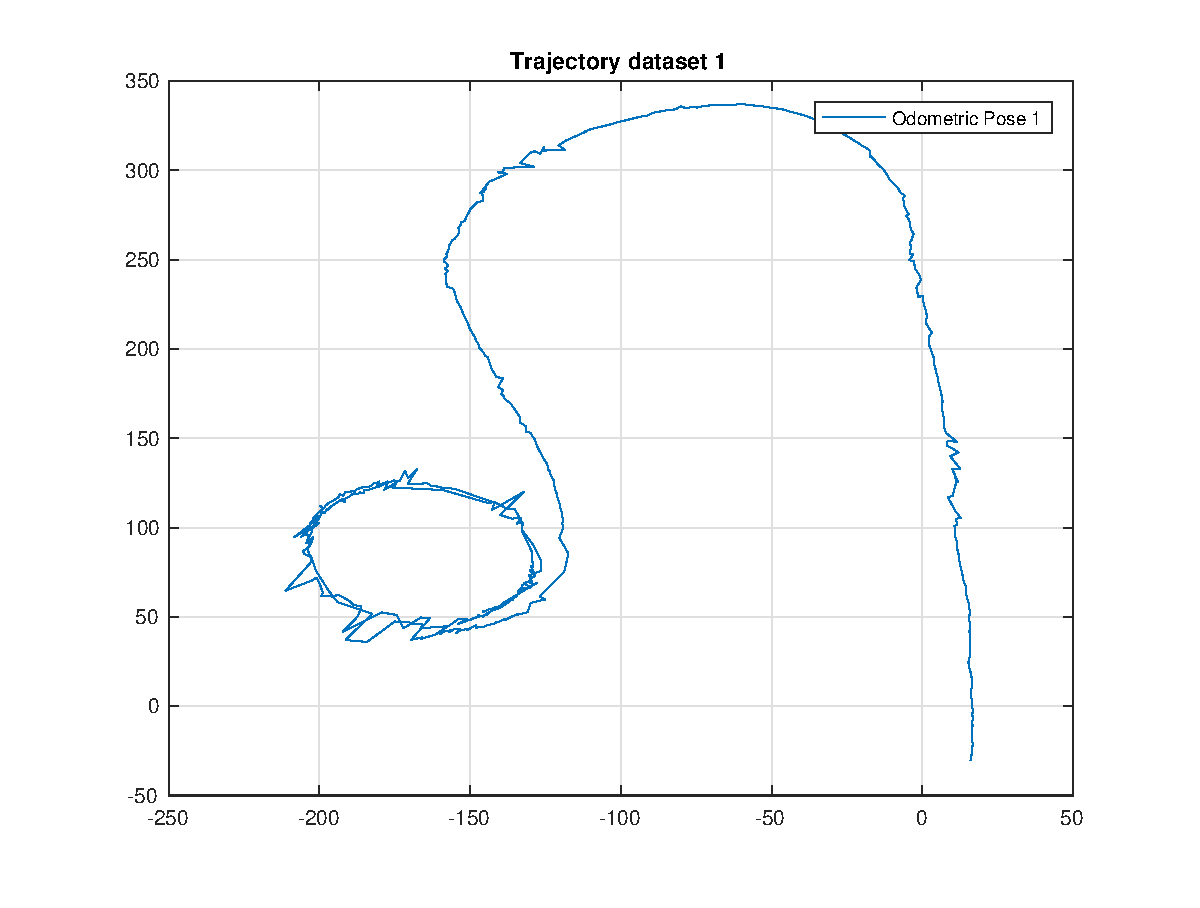
\includegraphics[scale=0.18]{trajectory_dataset_1.eps}} \,
\subfloat[][\emph{dataset 2}.]
   {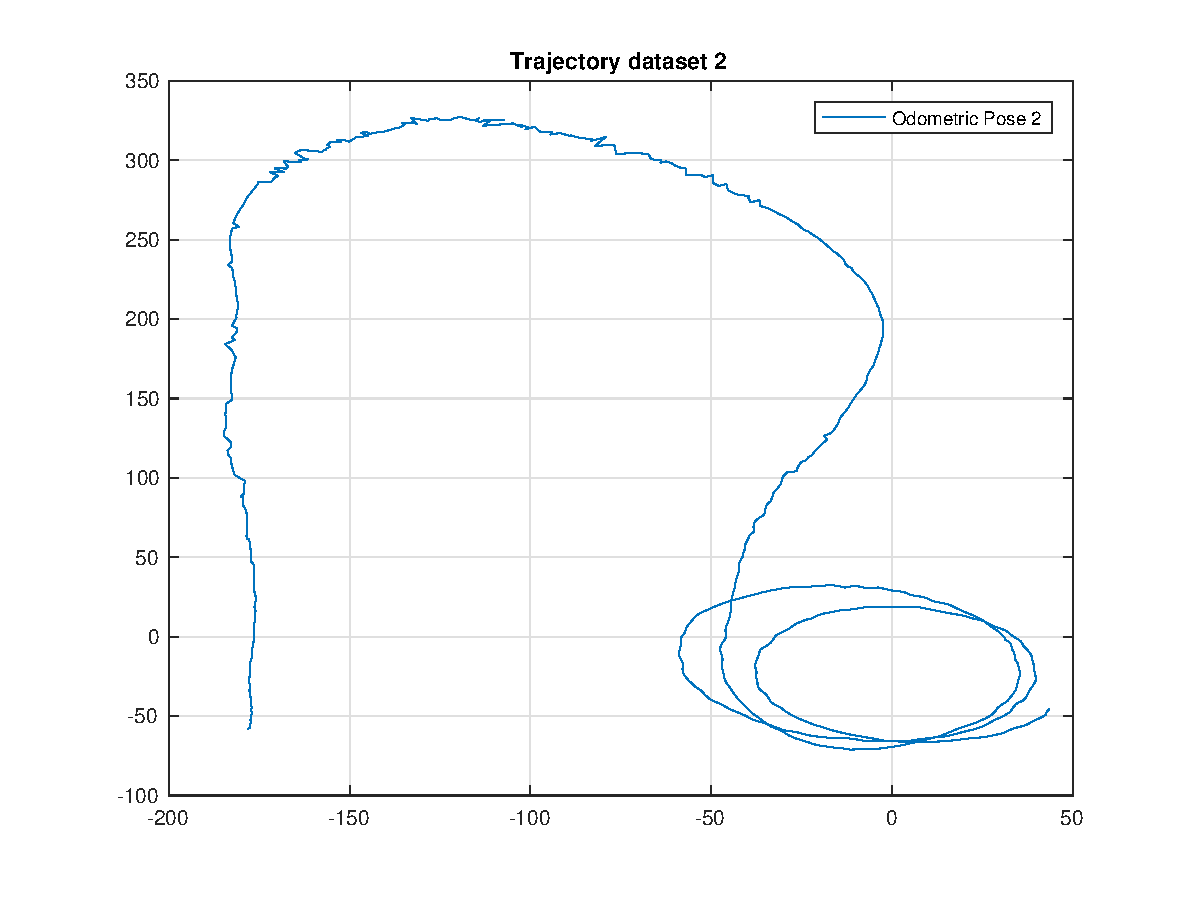
\includegraphics[scale=0.18]{trajectory_dataset_2.eps}} \\
\subfloat[][\emph{dataset 3}.]
   {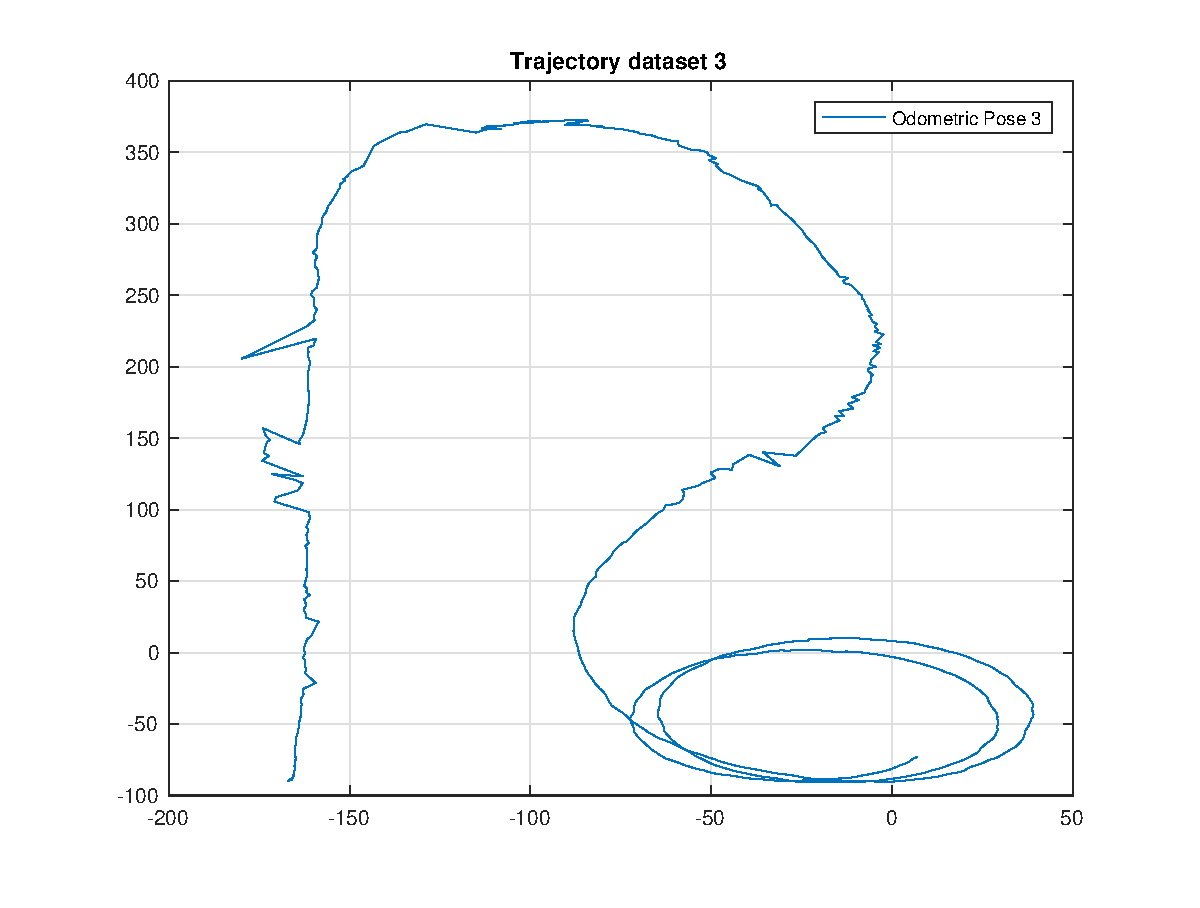
\includegraphics[scale=0.18]{trajectory_dataset_3.eps}} \,
\subfloat[][\emph{dataset 4}.]
   {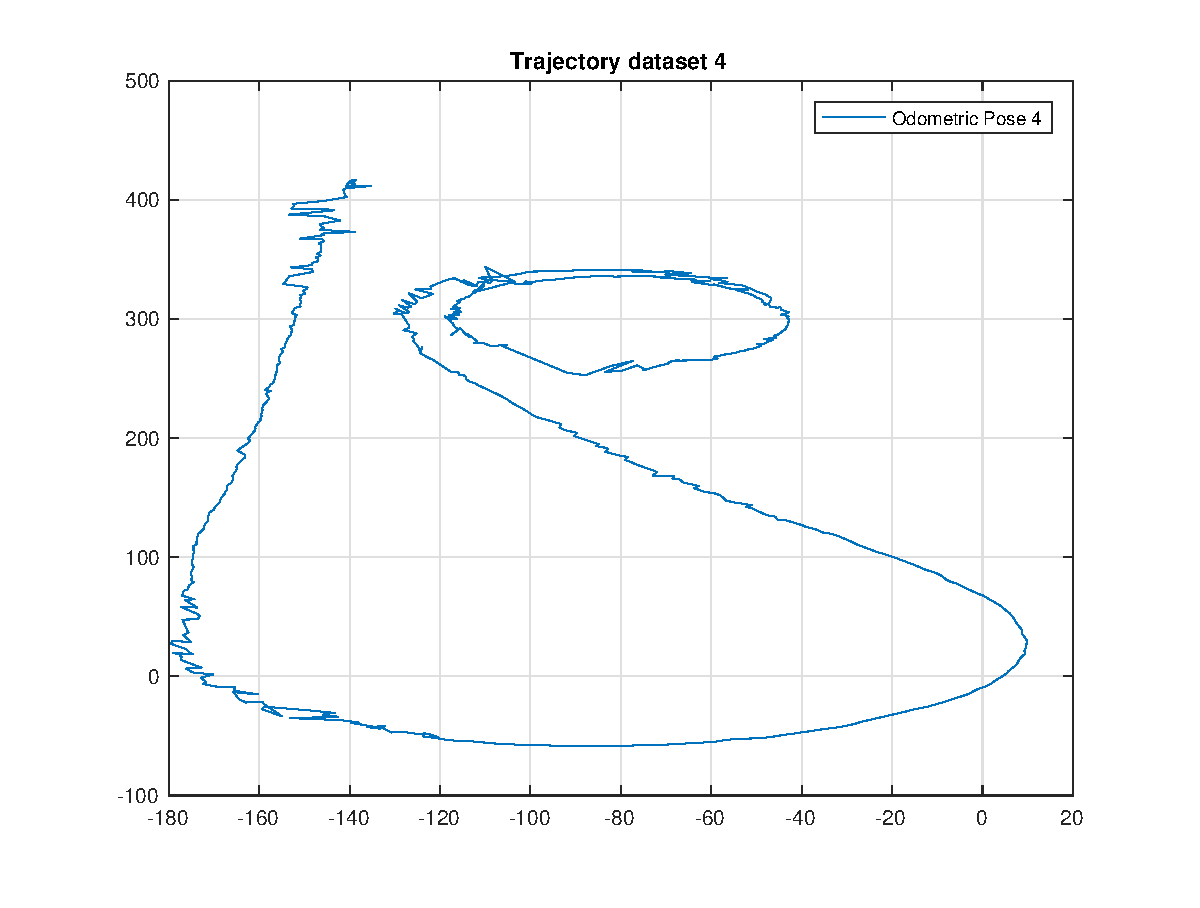
\includegraphics[scale=0.18]{trajectory_dataset_4.eps}}
\caption{Path from camera}
\label{fig:PathCamera}
\end{figure}

\begin{figure}[!h]
\centering
\subfloat[][\emph{dataset 1}.]
   {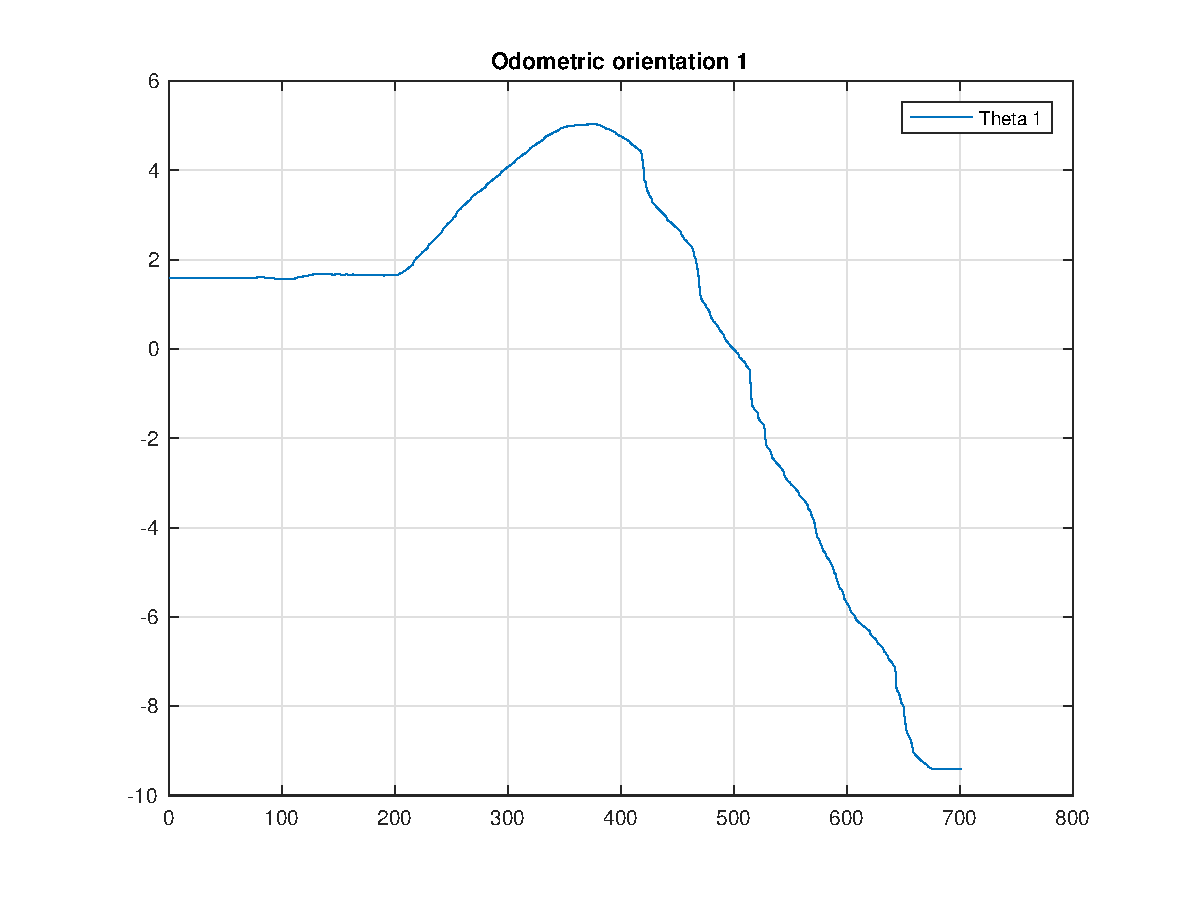
\includegraphics[scale=0.18]{angle_dataset_1.eps}} \,
\subfloat[][\emph{dataset 2}.]
   {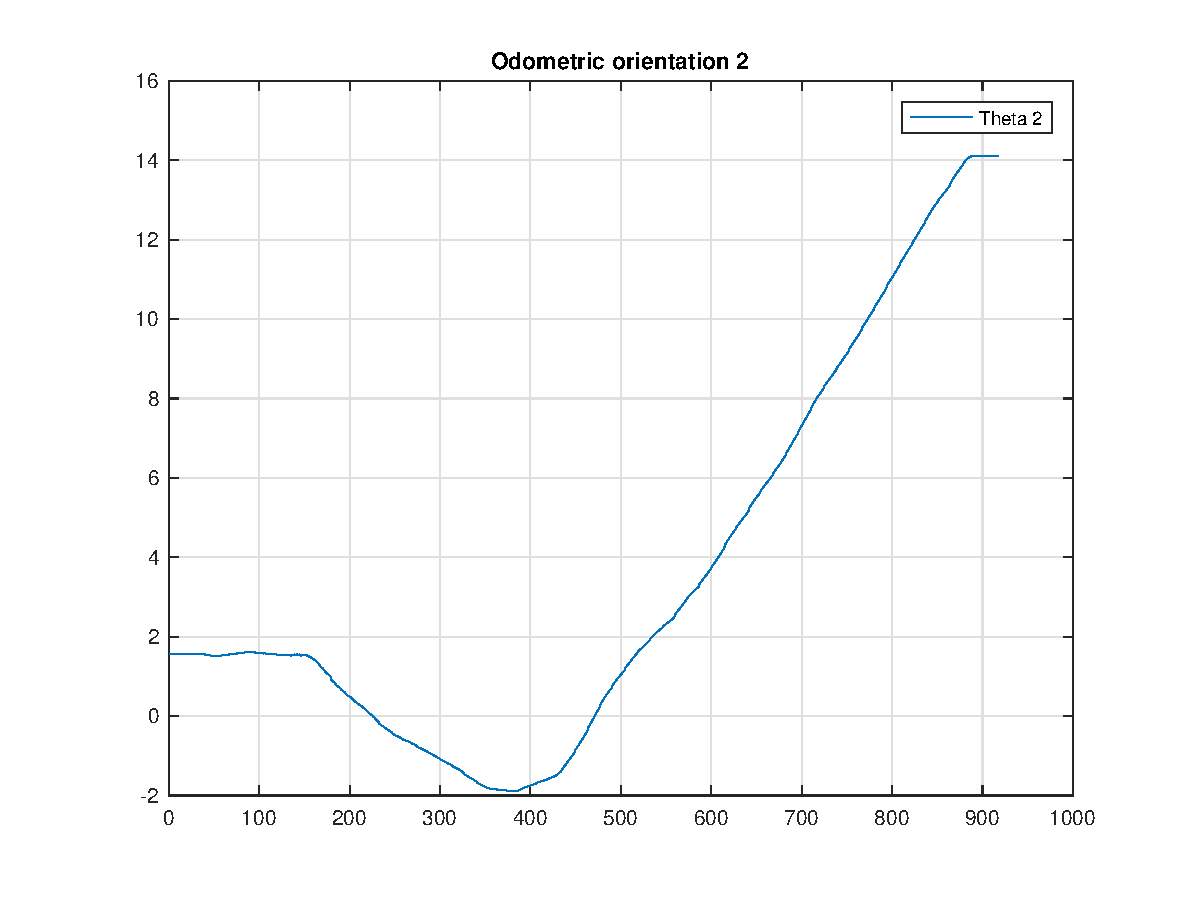
\includegraphics[scale=0.18]{angle_dataset_2.eps}} \\
\subfloat[][\emph{dataset 3}.]
   {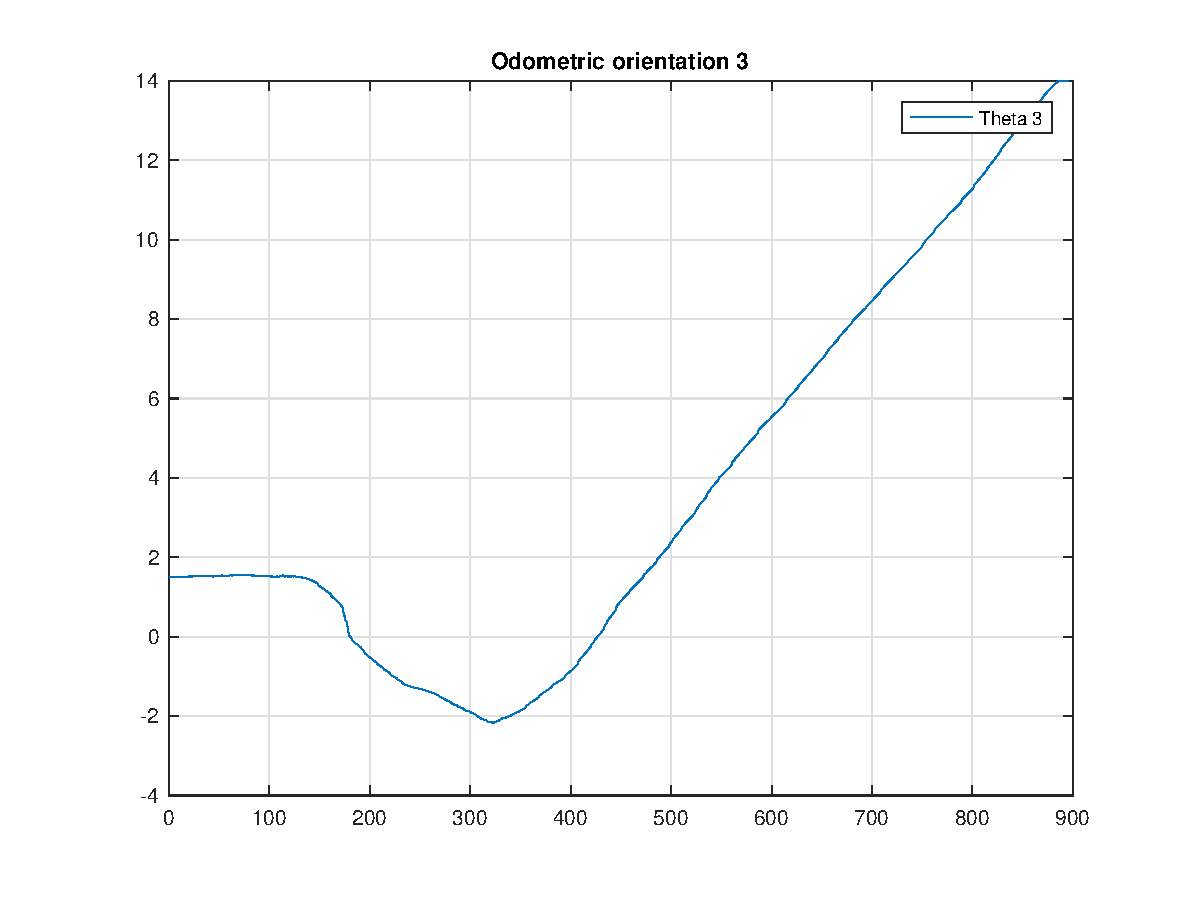
\includegraphics[scale=0.18]{angle_dataset_3.eps}} \,
\subfloat[][\emph{dataset 4}.]
   {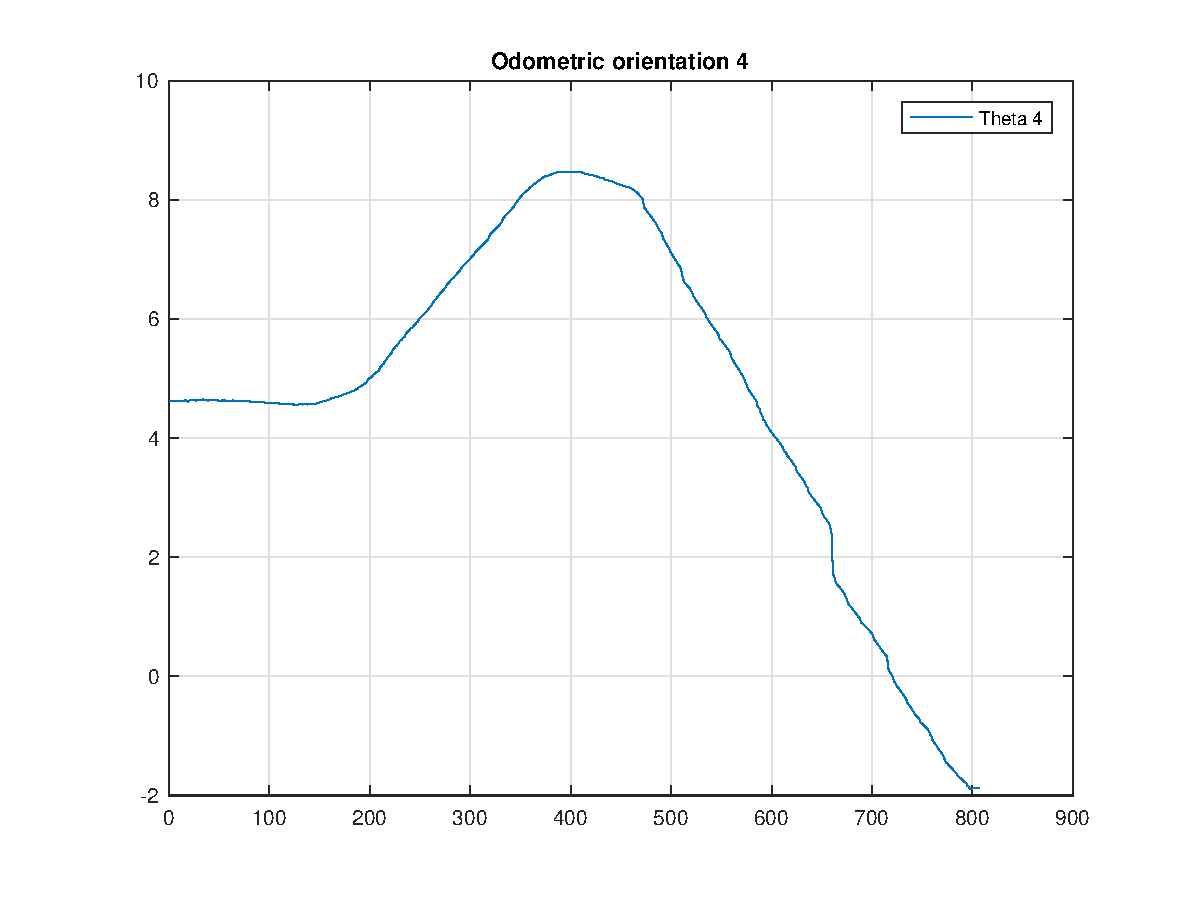
\includegraphics[scale=0.18]{angle_dataset_4.eps}}
\caption{Odometry orientation}
\label{fig:OdoOrientation}
\end{figure}

\begin{figure}[!h]
\centering
\subfloat[][\emph{dataset 1}.]
   {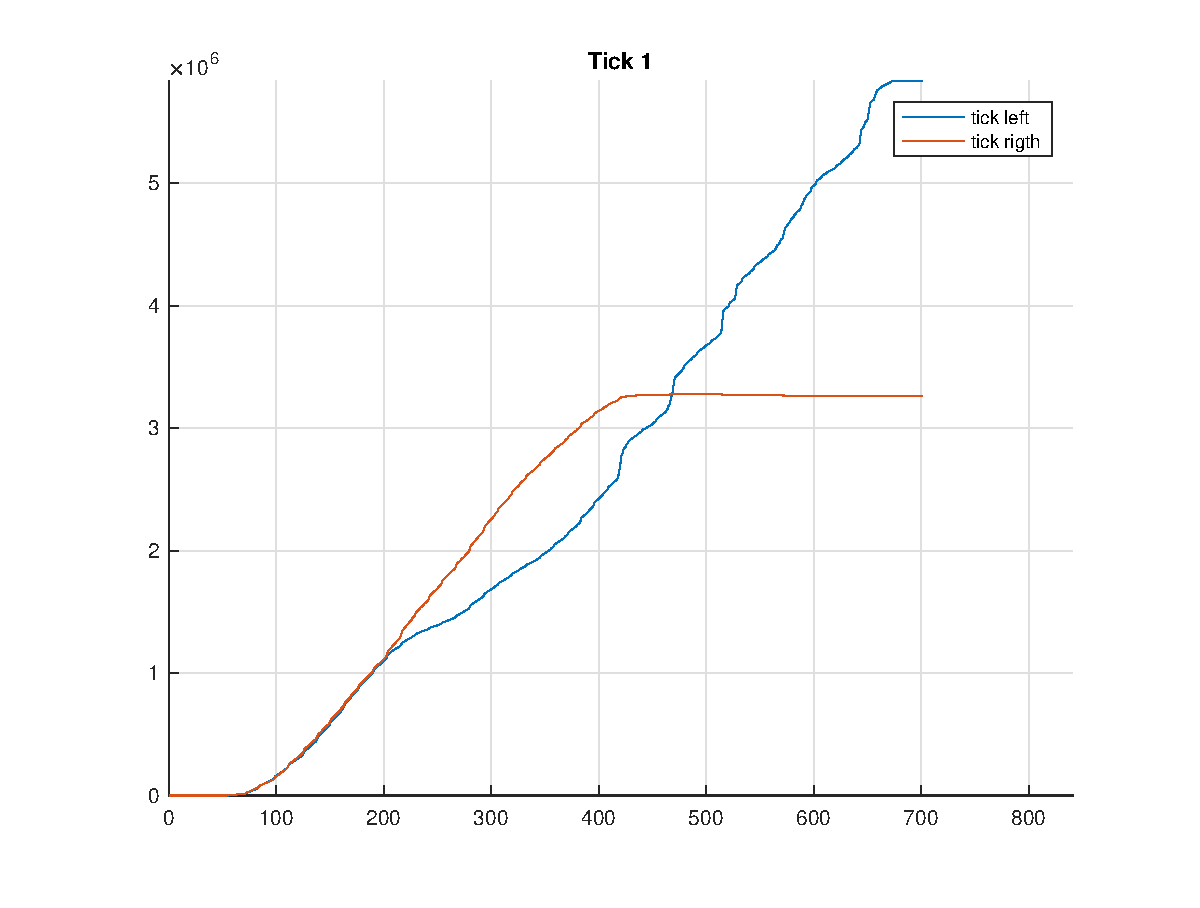
\includegraphics[scale=0.18]{tick_dataset_1.eps}} \,
\subfloat[][\emph{dataset 2}.]
   {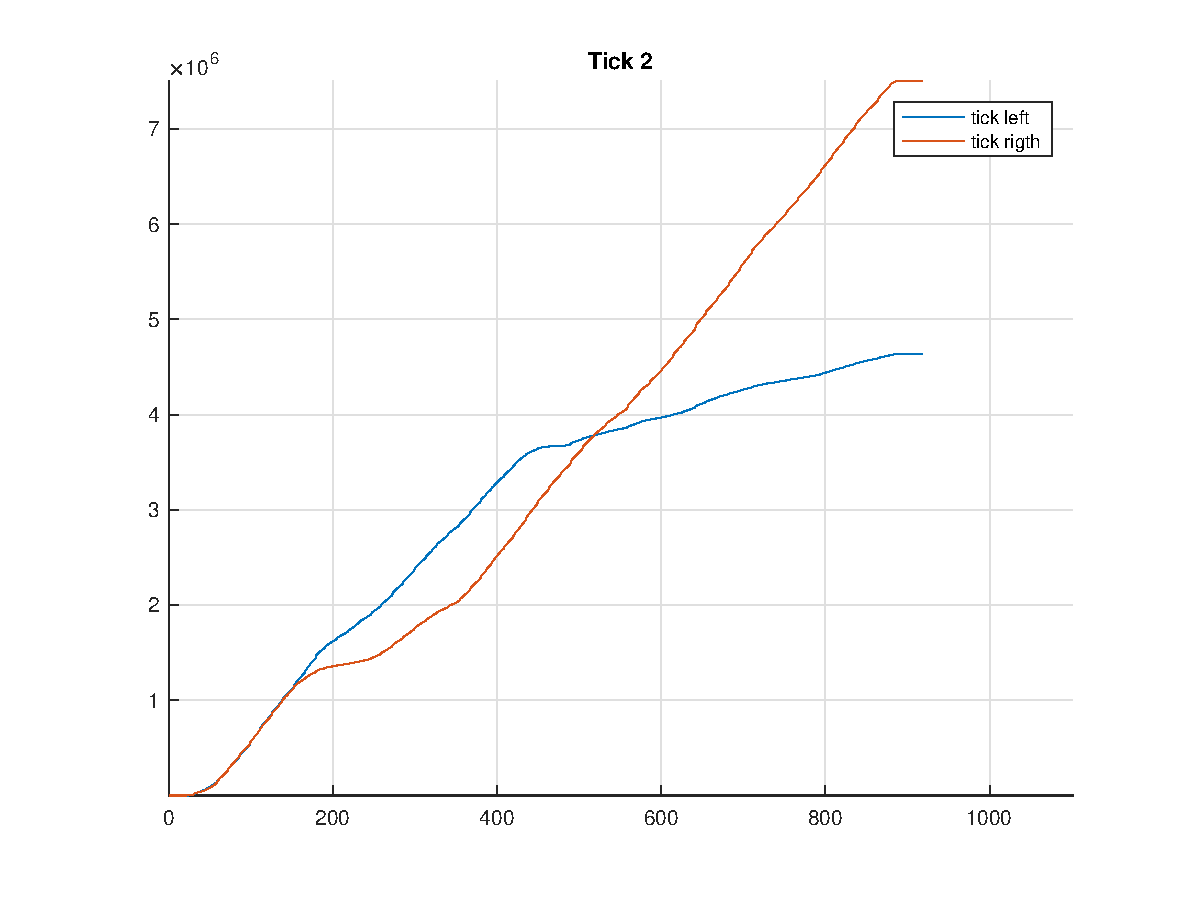
\includegraphics[scale=0.18]{tick_dataset_2.eps}} \\
\subfloat[][\emph{dataset 3}.]
   {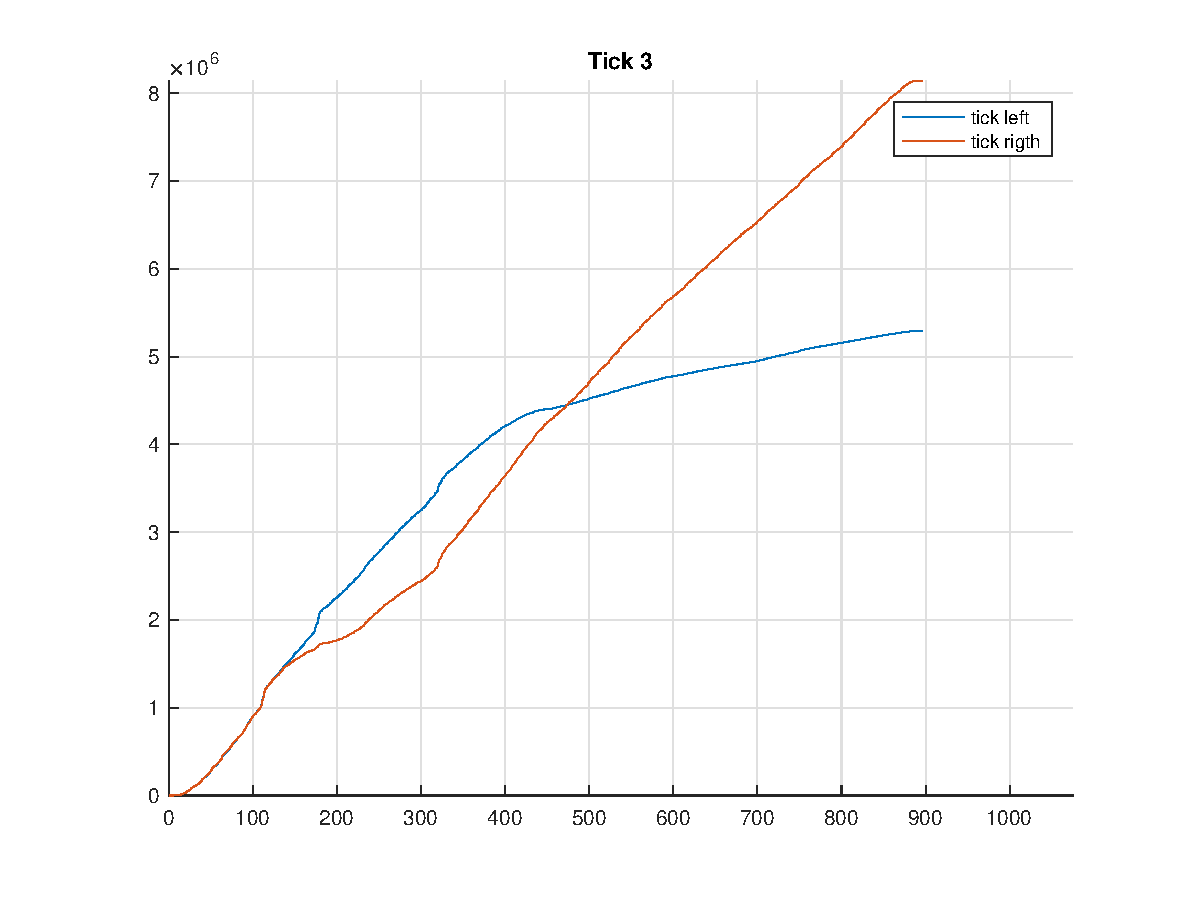
\includegraphics[scale=0.18]{tick_dataset_3.eps}} \,
\subfloat[][\emph{dataset 4}.]
   {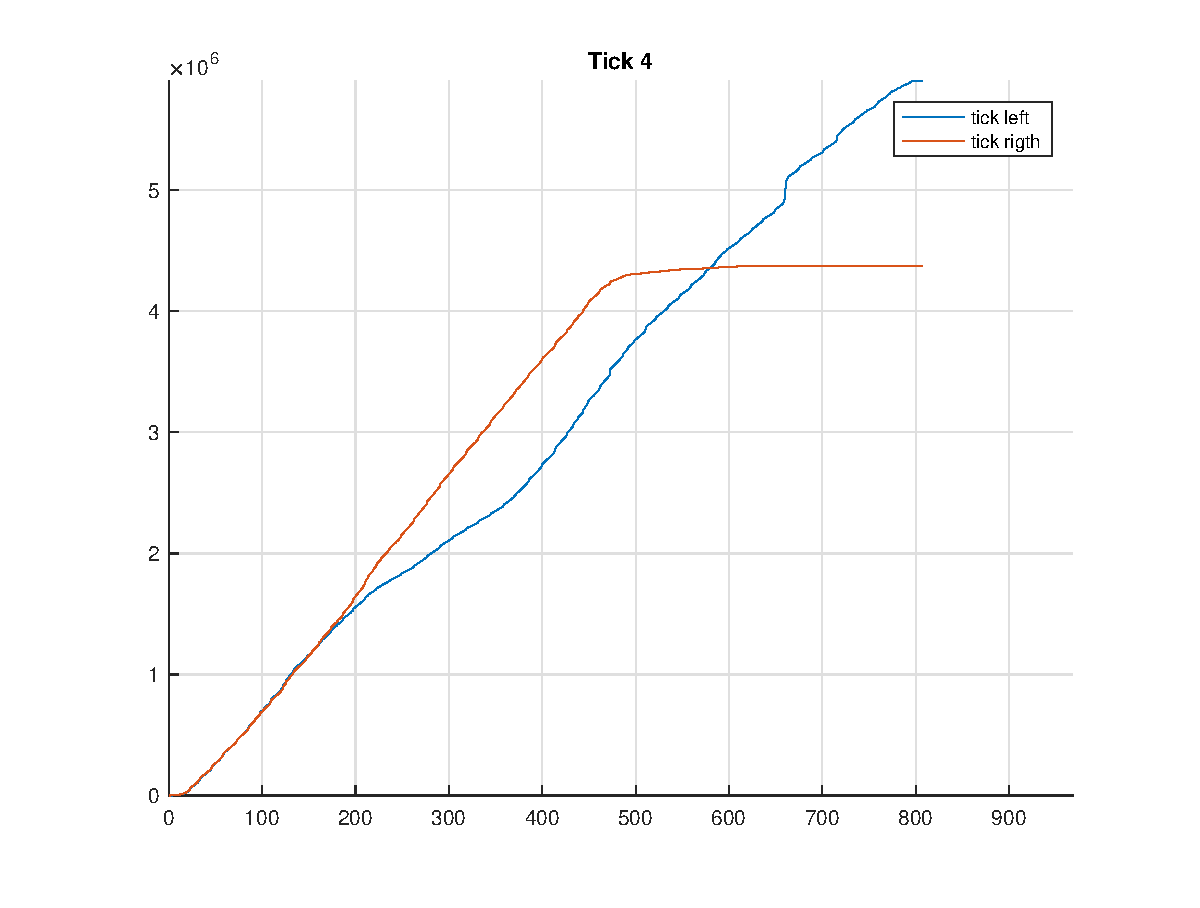
\includegraphics[scale=0.18]{tick_dataset_4.eps}}
\caption{Encoder trend}
\label{fig:tickPlot}
\end{figure}